\chapter{Representing the graph topology}

In this chapter, we propose a novel space-efficient approach to representing the graph topology.

%\section{Node and Edge IDs}
Source datasets typically identify nodes using unique identifiers (e.g., primary keys), which we term \emph{User Node IDs}. Let $V_U$ be the set of such User Node IDs. These identifiers may be strings or integers and generally do not fall within a predictable, compact range (like $\{0, \dots,  n-1\}$). Directly using these User Node IDs within graph data structures can be inefficient for storage and computation.

Therefore, we need to assign \emph{Internal Node IDs} to nodes. Let $V_I$ be the set of these Internal Node IDs. We aim for $V_I$ to be a compact set, specifically the fixed range $\{0,\dots , n - 1 \}$. We introduce a mapping $\mathrm{Id}_V: V_U \to V_I$ from these arbitrary User Node IDs to a compact set of Internal Node IDs.

While edges do not necessarily have a user identifier assigned, we still assign an Internal ID. Let $E_I$ be the set of these Internal Edge IDs, explicitly $E_I = \{0, \dots, m - 1\}$.

\problem{We need to provide our graph database with a map $\mathrm{Id}_{V}: V_U \to V_I$. Such a map should be bidirectional, allowing efficient computation of both $\mathrm{Id}_{V}$ and $\mathrm{Id}_{V}^{-1}$. The graph database should also be able to assign each edge $e \in E$ a numeric identifier $\mathrm{Id}_E(e) \in E_I$.}

Once our graph database is equipped with such mappings, we can revisit Definition~\ref{def:lpg} in terms of these internal IDs.

\begin{definition}
    A Labeled Property Graph (LPG) is a tuple
    \[
        G = (V_I, E, L, \mathrm{l}_V, \mathrm{l}_E, K, W, \mathrm{p}_V, \mathrm{p}_E),
    \]
    where:
    \begin{itemize}
        \item $V_I = \{0,\dots, n-1\}$ is the set of internal node IDs.
        \item $E \subseteq V \times V$ is a multiset of directed edges.
        \item $L$ is the set of labels.
        \item $K$ is the set of property keys.
        \item $W$ is the set of property values.
        \item $l_V: V_I \to L \cup \{\epsilon\}$ assigns an optional label to each node.
        \item $l_E: E_I \to L \cup \{\epsilon\}$ assigns an optional label to each edge.
        \item $p_V: V_I \times K \to W \cup \{\epsilon\}$ assigns properties to nodes, if defined.
        \item $p_E: E_I \times K \to W \cup \{\epsilon\}$ assigns properties to edges ids, if defined.
    \end{itemize}
\end{definition}

\section{Representing Node IDs}
Constructing an appropriate $\mathrm{Id}_V$ is equivalent to determining a suitable graph relabelling. While we will tackle that task in the following section, our current focus is on introducing two space-efficient data structures for storing $\mathrm{Id}_V$ and its inverse $\mathrm{Id}_V^{-1}$.
A trivial approach would be to keep two hash maps $\mathrm{Id}_V$ and $\mathrm{Id}_V^{-1}$, but this would lead to a significant storage overhead. 


\subsection{Permutation-based mapping}
We propose a compact data structure for mapping between User Node IDs and $V_I = \{ 0, \dots, n - 1\}$. It supports both integer and string keys, but offers better performance and compression ratios when keys are integers.

We call $\mathcal{K}eys$ the zero-indexed sorted array such that $\mathcal{K}eys[i]$ is the $i$-th User Node ID according to some total ordering over $V_U$ (e.g., the canonical ordering). The $\mathcal{K}eys$ array acts as an intermediate mapping from a $userID \in V_U$ to its index $i$ in the sorted sequence. We then define a permutation $\pi$ on $V_I$, i.e, the indices $\{0, \dots, n - 1\}$, such that $\mathit{userID} = \mathcal{K}eys[i] \implies \pi^{-1}(i) = \mathit{internalID}$. Such $\pi$ can be constructed as an invertible permutation as described in Section~\ref{sec:invperm} using $t = \lceil \log_2 n \rceil$ where $n = \#\mathcal{K}eys$. 

This setup allows us to compute both $\mathrm{Id}_V(\mathit{userID})$ and its inverse $\mathrm{Id}_V^{-1}$ (given the corresponding $\mathit{internalID}$) efficiently:
\begin{itemize}
    \item To compute $\mathrm{Id}_V(\mathit{userID})$  we first perform a binary search over $\mathcal{K}eys$ and find the index $i$ such that $\mathcal{K}eys[i] = \mathit{userID}$. We then map such an index to the corresponding $\mathit{internalID}$ through $\pi^{-1}$.
    \item $\mathrm{Id}_V^{-1}(\mathit{internalID})$ is computed as follows. We compute $i = \pi(\mathit{internalID})$ and then we get its corresponding key by accessing $\mathcal{K}eys[i]$.
\end{itemize}

Clearly, this scheme supports both integer and string-based User Node IDs. However, if User Node IDs are integers, the $\mathcal Keys$ array can be compressed using Elias–Fano encoding to save space. On the other hand, when User Node IDs in $V_U$ are strings, the scheme remains valid, with the only overhead being the cost of string comparisons during binary search in $\mathrm{Id}_V$.

\begin{theorem}\label{thm:map}
If $V_U$ consists of $n$ non-negative integers bounded by $u$, the proposed data structure serves $\mathrm{Id}_V$ in $O(\log n)$ time and $\mathrm{Id}_V^{-1}$ in constant-time, while taking at most  $n (7 + \log_2 u) + o(n)$ total bits of space.
\end{theorem}

\begin{proof}
$\mathrm{Id}_V$ requires performing a binary search over $Keys$, which takes $O(\log_2 n)$ time, and computing the inverse of the index returned by the binary search through $\pi^{-1}$, which takes $O(t) = O(\log_2 n)$ time. The time complexity of $\mathrm{Id}_V^{-1}$ is given by accessing first $\pi$ and then the $i$-th key, both constant-time operations.

Finally, the space taken by the map is the sum of the space taken by $\mathcal {Keys}$ and $\pi$.
If encoded with Elias-Fano, $\mathcal Keys$ requires at most $n (2 + \lceil \log_2 u / n \rceil) + o(n)$ bits, while $\pi$ requires $n \lceil \log_2 n \rceil + n + n \frac{2}{t + 1} \lceil \log_2 n \rceil + o(n)$ bits.
The sum of these 2 quantities can then be rewritten as follows: 
\[
\begin{aligned}
    &n (2 + \lceil \log_2 u / n \rceil) + o(n) + n \lceil \log_2 n \rceil + n + n \frac{2}{t + 1} \lceil \log_2 n \rceil + o(n) \\
    &= 3n + n\lceil \log_2 (u / n) \rceil + n \lceil \log_2 n \rceil + n \frac{2}{\lceil \log_2 n \rceil + 1} \lceil \log_2 n \rceil + o(n) \\
    &\le 3n + n\lceil \log_2 (u / n) \rceil + n \lceil \log_2 n \rceil + 2n + o(n) \\
    &= n ( 5 + \lceil \log_2 (u / n) \rceil + \lceil \log_2 n \rceil ) + o(n) \\
    &\le n ( 5 + \log_2 u - \log_2 n + 1 + \log_2 n + 1) + o(n) \\
    &= n (7 + \log_2 u) + o(n)
\end{aligned}
\]

\end{proof}

% You might want to rephrase this
Alternatively, a similar result could be achieved by using two Minimal Ordered Perfect Hash (MOPH) functions \cite[Section~8.6]{PearlsAE}, with negligible additional space overhead. Such an approach would yield an optimal $O(1)$ time complexity for computing both $\mathrm{Id}_V$ and its inverse $\mathrm{Id}_V^{-1}$. We opted instead for the permutation-based method due to its implementation simplicity. Moreover, this approach already provides sufficient performance guarantees. While the $O(\log n)$ complexity for computing $\mathrm{Id}_V$ is suboptimal, in practice the overhead is minimal since we query $\mathrm{Id}_V$ infrequently—for example, only at the beginning of a traversal such as a BFS from a given node. On the other hand, computing $\mathrm{Id}_V^{-1}$ is a more frequent operation (e.g., to translate Internal Node IDs back into User IDs throughout the visit) and is conveniently carried out in optimal $O(1)$ time by our proposed scheme.

\subsection{FM-Index-based mapping}\label{sec:FMIdxMapping}

We now propose another approach that aggressively compresses the underlying data, with the drawback of having more expensive retrievals.

We consider the case where the User Node IDs are strings. This is not limiting since integer keys can be easily encoded as strings as well. Let then $\xi$ be a delimiter such that $\xi \not \in \Sigma$  where $\Sigma$ is the alphabet in which $V_U$ elements are drawn.

Let \(key_i\) denote the User Node ID such that \(\mathrm{Id}_V(key_i) = i\). We define the string \(\bar{\mathcal{T}}\) as follows:

\[
\bar{\mathcal{T}} = \xi \cdot key_0 \cdot \xi \cdot key_1 \cdot \xi \cdots \xi \cdot key_{n - 1} \cdot \xi
\]

The structure \(\mathcal{T}\) is then the representation of \(\bar{\mathcal{T}}\) using a CSA based on Huffman-shaped Wavelet Trees.

Finally, we build a (sparse) binary-vector $\mathcal B$ such that $\mathcal B[i] = 1 \iff \bar{\mathcal{T}} [i] = \xi$.

Using $\mathcal{T}$ and $\mathcal{B}$, we can implement $\mathrm{Id}_V$ and $\mathrm{Id}_V^{-1}$ as follows:
\begin{align*}
  \mathrm{Id}_V(\mathit{userID})
    &= \operatorname{rank}_{\mathcal{B}}\left(
          \operatorname{locate}_{\mathcal{T}} \left(
            \xi \cdot \mathit{userID} \cdot \xi
          \right) + 1
        \right) - 1 \\
\\
  \mathrm{Id}_V^{-1}(\mathit{internalID})
    &= \operatorname{extract}_{\mathcal{T}} \bigl(
        \begin{array}[t]{l}
          \operatorname{select}^1_{\mathcal{B}}(\mathit{internalID} + 1) + 1, \\[0.2em]
          \operatorname{select}^1_{\mathcal{B}}(\mathit{internalID} + 2)
        \end{array}
      \bigr)
\end{align*}


The main advantage of this approach lies in its compactness: both $\mathcal{T}$ and $\mathcal{B}$ can be represented succinctly, with entropy-compressed representations delivering space close to the information-theoretic lower bound. However, the cost of these compact representations is that querying is more expensive compared to the permutation-based implementation, especially for $\mathrm{Id}_V$, which requires a full pattern search.

\section{Compressing the graph structure}

The preceding section has laid the groundwork necessary for efficiently representing Node IDs. This section now focuses on tackling the related challenge of effectively representing the adjacency lists that encode graph topology. Precisely, we need a data structure that compactly stores neighborhoods of nodes (adjacency information), and we must identify a suitable scheme for assigning internal Node IDs in a manner conducive to succinct representation.

When designing such a mechanism, three essential considerations arise:

\begin{enumerate}
    \item The adjacency lists must allow constant-time query operations, i.e., given a node \(v\) and an integer index \(i\), access to the $i$-th neighbor $N_v(i)$ should be supported in $O(1)$ time. We might also be interested in supporting efficient backwards queries (i.e., getting the parents of a given node).
    \item The solution must achieve good compression regardless of the nature of the graph. Indeed, GDBs are not specifically designed for one single domain (e.g., social networks), so we aim to guarantee good compression rates on both sparse and dense graphs.
    \item The node relabeling strategy should be carefully chosen to optimize compression. Intuitively, assigning adjacent nodes close internal IDs often results in more-compressible adjacency sequences.
\end{enumerate}

\subsection{Limitations of current approaches}

Figure~\ref{fig:preliminar_analysis} illustrates the compression rates of existing solutions presented in Section~\ref{sec:graph-compression} on the topology of the test datasets described in Chapter~\ref{chap:datasets-graphs}.

\begin{figure}[h]
    \centering
    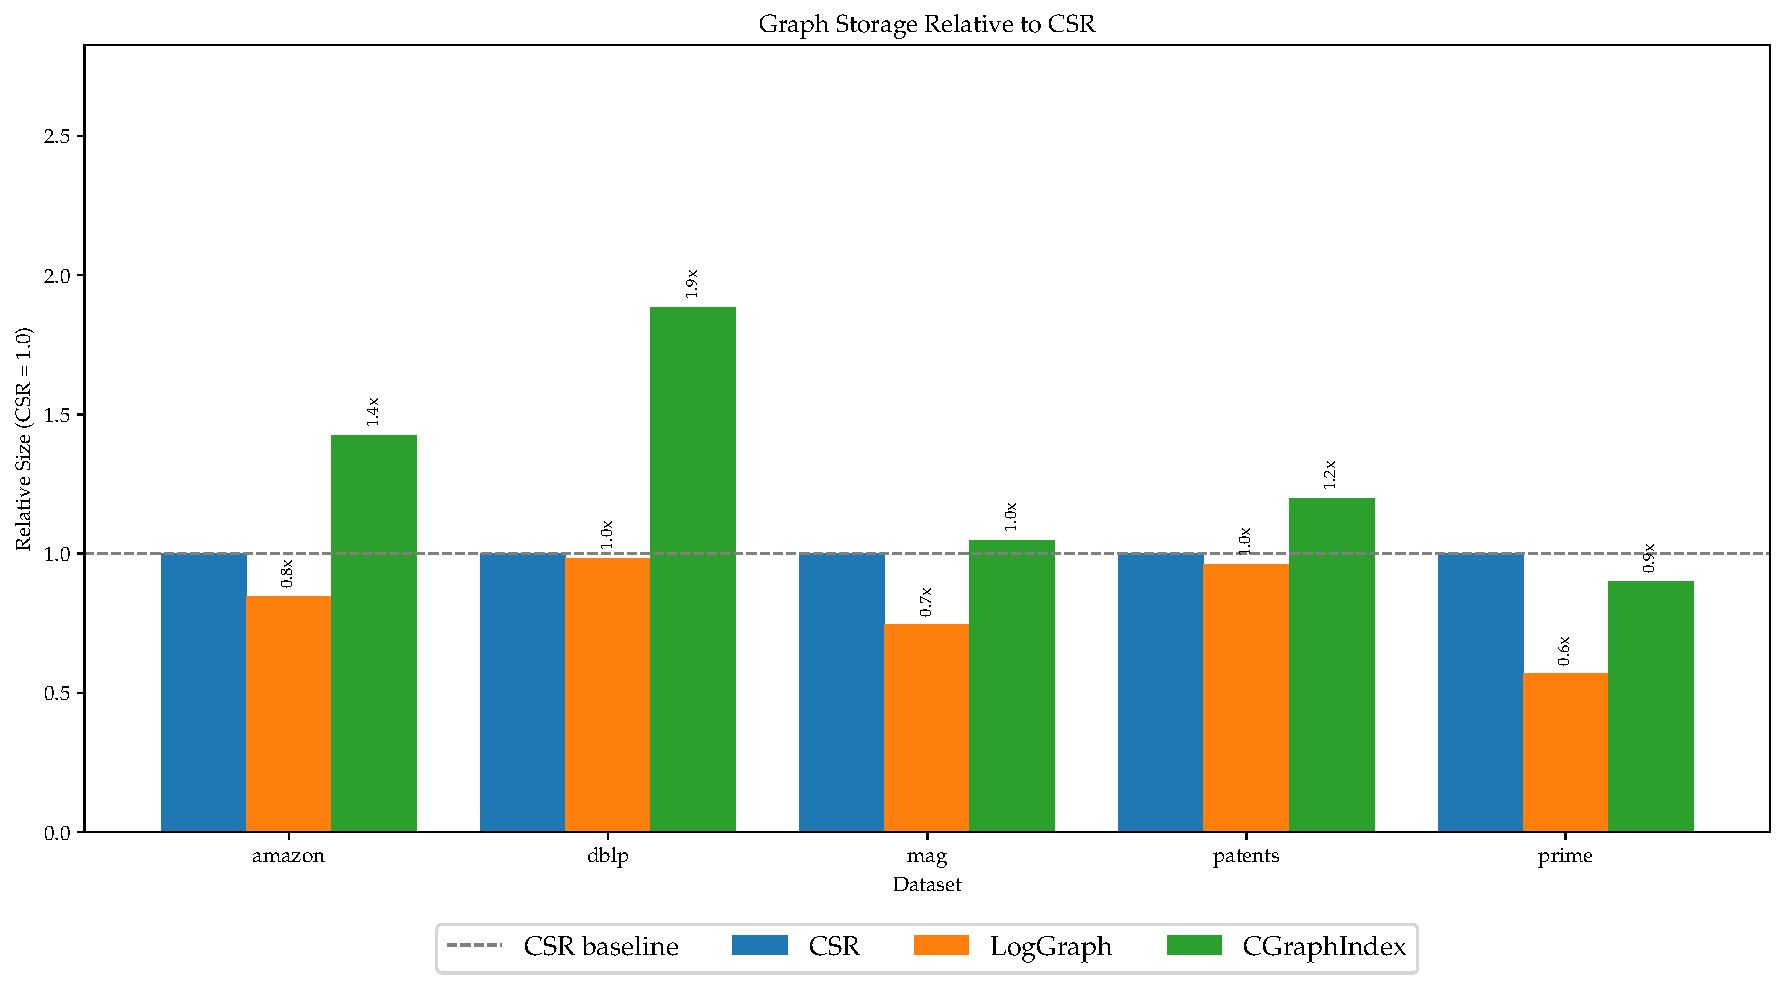
\includegraphics[width=\linewidth]{plots/adj_size_preliminary.pdf}
    \caption{
Comparison of storage sizes across different graph representations (CSR [Compressed Sparse Row], LogGraph, and CGraphIndex), normalized to the CSR size for each dataset (CSR = 1.0 baseline).
}
    \label{fig:preliminar_analysis}
\end{figure}


We observe that the compression performance of CGraphIndex is consistently worse than LogGraph, whereas LogGraph achieves similar or better performance than CSR when the graphs exhibit dense connectivity. However, given the simplicity of CSR's design and the fact that most labeled graphs in GDBs applications are sparse, we believe there is room for achieving a solution that is easy to implement and effective in space/time performance.

Driven by these insights, we take the CSR scheme as our baseline and introduce further optimizations, leveraging assumptions we can make on the underlying data. Concretely, we focus on the compression of the concatenated neighborhoods $\mathcal A$. Without loss of generality, we assume that each neighborhood $N_v$ is sorted in increasing order within $\mathcal A$, and we propose a technique to compress it efficiently, exploiting possible clusters within.  Actually, such a technique can be applied to any integer sequence and, in the case of $\mathcal{A}$, if each neighborhood $N_v$ is compact (i.e., $\max N_v - \min N_v$ is small),  then the neighborhoods form clusters.

Finally, we argue that an appropriate graph relabelling strategy can enhance the formation of clusters in $\mathcal{A}$, thus maximizing the effectiveness of our approach.

\subsection{A cluster-aware integer compression technique}
Let $\mathcal S$ be an arbitrary sequence of $l$ non-negative integers bounded by $u > 0$, and  $b = \lceil \log_2 u \rceil$ the minimum number of bits necessary to represent every element in $\mathcal S$.

Our compression scheme is based on the observation that clustered sequences of integers frequently share common prefixes in their binary representation. We exploit this fact by splitting each integer into two parts on a chosen \emph{split point} $0 \le h \le b$. We denote the $h$ most significant bits with \(s_i^+\), and the remaining $b - h$ bits with $s_i^-$. 
Additionally, we maintain a bit-vector $\mathcal{B}$ of length $l$ recording whether consecutive elements share identical $s_i^+$ values. Formally, the bit-vector $\mathcal{B}$ is defined as:
\begin{equation*}
    \mathcal B [i] = \begin{cases}
    1 & i = 0 \lor s_{i - 1}^+ \ne s_{i}^+ \\
    0 & \text{otherwise}
    \end{cases}.
\end{equation*}
Intuitively, a bit set to 1 indicates the start of a new cluster in the high bits sequence. Consequently, we only explicitly store high-bit values corresponding to positions with a 1-bit in $\mathcal B$. Thus, the high sequence $\mathcal H$ stores exactly as many integers as there are ones in $\mathcal{B}$, while the low bits $\mathcal L$ always store low-bit values for all $l$ integers.

\begin{lemma}
If $\mathcal B$ is equipped with a rank-support data structure, we can implement $\text{Access}(\mathcal S, i)$ to reconstruct $s_i$ from $\mathcal L$, $\mathcal H$, and $\mathcal B$ in $O(1)$ time.
\end{lemma}

\begin{proof}
We define the access function as:
\begin{equation*}
    \text{Access}(\mathcal S, i) = \mathcal H[\text{rank}_{\mathcal B}(i + 1) - 1] \times 2^h + \mathcal L[i].
\end{equation*}
Clearly, this expression can be evaluated in $O(1)$ time assuming that $\mathcal B$ supports $\text{rank}$ queries in constant time.

To establish correctness, we need to demonstrate two properties: (i) $\mathcal L[i] = s_i^- $, and (ii) $ \mathcal H[\text{rank}_{\mathcal B}(i+1) -1] = s_i^+ $. The first property follows immediately from the construction of the array $\mathcal  L $, which explicitly stores the lower $ h $ bits of each element. The second property can be proven using mathematical induction, as it reflects the mapping of positions in $ \mathcal B $ to entries in $\mathcal H $.
\end{proof}



We can also observe that for the special case $h= 0$, the proposed scheme is fully equivalent to bitpacking, therefore, we can avoid storing $\mathcal B$ in such a case. We summarize these results about the space occupancy in the following theorem.
\begin{theorem}\label{thm:space}
    For any split point $h$, the number of bits required by the proposed encoding scheme is
\begin{equation*}
    \mathrm{Space}(\mathcal S, h) = \begin{cases}
        \mathrm{rank}_{\mathcal B}(l) \times h + l \times (\lceil \log_2 u \rceil - h) + l + g(l) & h > 0 \\
        l \times \lceil \log_2 u \rceil  & h = 0
    \end{cases}
\end{equation*}
where $g(l)$ is typically a $o(l)$ function due to the $\mathcal B$'s rank support overhead.\footnote{In our implementation, we use  SDSL \texttt{rank\_support\_v5} and $g(l) \approx 0.0625\: l$.}
\end{theorem}

Such a quantity can also be computed in linear time without explicitly constructing $\mathcal H, \mathcal L$, and $\mathcal B$. Indeed,  we just have to count the number of 1s we would have in $\mathcal B$ which can be done by traversing $\mathcal S$.

We are now interested in choosing the split point $ h $ that minimizes the overall space usage of the encoding.
\begin{definition}
    We define the optimal split point $h^*$ of a sequence $\mathcal{S}$ the quantity
\begin{equation*}
    h^*(\mathcal S) = argmin_{0 \le h \le b} \ \mathrm{Space}(\mathcal S,  h).
\end{equation*}
\end{definition}

Clearly, we are always interested in using $ h^*(\mathcal{S}) $ as a split point; therefore, when omitted, the representation will implicitly refer to this optimal split. Let we start with this simple theorem.

\begin{theorem}
The proposed representation of a sequence $\mathcal S$ can be built in $O(l \times \log_2 u)$ time and $O(1)$ additional space.
\end{theorem}

\begin{proof}
    To construct the proposed representation, we iterate over possible partitioning parameters $0 \leq h \leq \lceil \log_2 u \rceil$. For $h = 0$, computing $\mathrm{Space}(\mathcal S, h)$ is trivial, while for each candidate value of $h > 0$, we need to compute $\mathrm{rank}_{\mathcal B}(l)$, which is the only term of $\mathrm{Space}(\mathcal S, h)$ that depends on the split given by $h$ on $\mathcal S$. We can do that by noting that the number of 1s in $\mathcal S$ equals to the number of elements $s_i$ in $\mathcal S$ such that $i = 0 \lor s_i^+ \ne s_{i -1}^+$. This computation takes $O(l)$ time per value of $h$ and $O(1)$ space. Since there are at most $b= \lceil \log_2 u \rceil$ such values, the total time to find the optimal split point $h^*$ (that minimizes space) is $O(l \times \log_2 u)$.

    Once $h^*$ is determined, we construct $\mathcal L$, $\mathcal H$, and $\mathcal B$ in $O(l)$ time. Therefore, the total time complexity remains $ O(l \times \log_2 u) + O(l) = O(l \times \log_2 u) $.
\end{proof}


In most practical settings, such an algorithm is already fast given its low memory footprint and the fact that we scan $\mathcal S$ linearly, thus with a \emph{cache-oblivious} behaviour. However, we can come up with a $O(l + \log_2 u)$ time construction algorithm, as stated in the following theorem.

\begin{theorem}
    It exists an algorithm taking $O(l + \log_2 u)$ time that finds $h^*(\mathcal S)$ and hence constructs the compressed representation of $\mathcal S$. Furthermore, the algorithm requires $O(\log_2 u)$ words of additional space.
\end{theorem}
\begin{proof}
Let \( b = \lceil \log_2 u \rceil \). We define the function \(\mathrm{LCP}(j)\) as the length of the longest common prefix between the \(b\)-bit binary representations of elements \( s_{j-1} \) and \( s_j \), for \( j \in \{1, \dots, l-1\} \). We compute each \(\mathrm{LCP}(j)\) in constant time by using a bitwise XOR followed by a count leading zeros instruction (e.g., \texttt{clz(s\(_{j-1}\)\(\oplus\)s\(_j\))}), treating the special case \(s_{j-1}=s_j\) as \(\mathrm{LCP}(j)=b\). For the sake of simplicity, we assume that the \texttt{clz} instruction counts the number of leading zeros within the fixed-width $b$-bit representations of the integers in $\mathcal S$ — that is, with each number zero-padded to $b = \lceil \log_2 u\rceil$ bits — rather than over the full machine word size.

Given $\mathrm{LCP}(j)$, for every $j \in \{1, \dots, l-1\}$, we then store its frequency in an array $\mathcal{F}[0,b]$, so that $\mathcal{F}[k]$ holds the number of indices $j$ such that $\mathrm{LCP}(j)=k$. The computation of $\mathcal{F}$ can be easily performed when computing the array $\mathrm{LCP}$ so in overall $O(l+b) = O(l)$ time.

Next, we iterate over the possible values of $h \in \{0, 1, \dots, b\}$ in order to find the optimal split point. To do that, we need to compute $\mathrm{Space}(\mathcal S, h)$. For $h = 0$, this is straightforward as it is equal to $b \times l$, while for $h >0$ we need to determine $\mathrm{rank}_{\mathcal{B}}(l)$ for such $h$, which is the number of 1s in the binary vector $\mathcal{B}$ that would be built using such split point $h$. Let this be $R_h$.

According to the definition of $\mathcal{B}$:
\begin{equation*}
    R_h = \mathcal{B}[0] + \sum_{j=1}^{l-1} \mathbbm{1}_{s_{j-1}^+ \neq s_j^+}.
\end{equation*}
Since $\mathcal{B}[0]=1$ and $s_{j-1}^+ \neq s_j^+$ if and only if $\mathrm{LCP}(j) < h$, we have:
\begin{equation*}
    R_h = 1 + \sum_{j=1}^{l-1} \mathbbm{1}_{\mathrm{LCP}(j) < h}.
\end{equation*}
Using the frequency array $\mathcal{F}$, this sum can be efficiently calculated:
\begin{equation*}
    R_h = 1 + \sum_{k=0}^{h-1} \mathcal{F}[k].
\end{equation*}
We can compute then all $R_h$ values iteratively. We detail the whole procedure to find $h^*(\mathcal S)$ in Algorithm~\ref{alg:find_optimal_h}.

\begin{algorithm}[H] % Use [H] for "here" placement if desired and if float package is loaded
\caption{Find Optimal Split Point $h^*$}
\label{alg:find_optimal_h}
\begin{algorithmic}[1]
\Require Sequence \(\mathcal{S} = (s_0, \dots, s_{l-1})\); overhead function \(g(l)\).
\Ensure Optimal split point \(h^*\).

\State \( b \gets \lceil \log_2 (\max \mathcal S + 1) \rceil \)
\State Initialize frequency array \(\mathcal{F}[0 \dots b-1] \gets 0\)

\Comment{Populate frequency array \(\mathcal{F}\)}
\For{\(j \gets 1\) \textbf{to} \(l - 1\)}
    \If{\(s_{j-1} \ne s_j\)}
        \State \(\ell \gets \texttt{clz}(s_{j-1} \oplus s_j)\)
        \State \(\mathcal{F}[\ell] \gets \mathcal{F}[\ell] + 1\)
    \EndIf
\EndFor

\Comment{Find optimal split point \(h^*\)}
\State \(\text{min\_space} \gets l \cdot b\), \quad \(h^* \gets 0\), \quad \(R_h \gets 1\)
\State \(\text{prefix\_sum} \gets 0\)
\For{\(h \gets 1\) \textbf{to} \(b \)}
    \State \(\text{prefix\_sum} \gets \text{prefix\_sum} + \mathcal{F}[h - 1] \)
    \State \(R_h \gets 1 + \text{prefix\_sum}\)
    \State \(\text{curr\_space} \gets R_h \cdot h + l \cdot (b - h) + l + g(l)\)
    \If{\(\text{curr\_space} < \text{min\_space}\)}
        \State \(\text{min\_space} \gets \text{curr\_space}\)
        \State \(h^* \gets h\)
    \EndIf
\EndFor
\State \Return \(h^*\)
\end{algorithmic}
\end{algorithm}

The second for-loop in Algorithm~\ref{alg:find_optimal_h} runs $b-1$ times. Each step within this loop takes constant time. Therefore, determining the $R_h$ and $\mathrm{Space}(\mathcal{S}, h)$ for all $h \in \{1, \dots, b\}$ takes $O(b)$ time, after the initial $O(l+b)$ LCP and frequency computation.

Once $h^*$ is determined, the actual data structures $\mathcal{L}$, $\mathcal{H}$, and $\mathcal{B}$ (along with its rank support) are constructed. This involves a single pass over the input sequence $\mathcal{S}$ to extract the relevant bit parts for $\mathcal{L}$ and to determine $\mathcal{B}$, and then to populate $\mathcal{H}$. This construction takes $O(l)$ time.

Therefore, the total time complexity to find $h^*$ and build the proposed representation is $O(l+b) + O(b) +  O(l) = O(l+b)$. Regarding space complexity, the algorithm stores the array \(\mathcal F\) of length \(b + 1\) and a constant number of auxiliary variables, thus $O(b)$ extra space.
\end{proof}



Next, we may argue that the choice of one single optimal split point $h^*$ for a possible long sequence $\mathcal S$ is a global optimal choice, which doesn't guarantee that each cluster is compressed optimally. Indeed, clusters might have different lengths and distributions. To address this inefficiency, we can uniformly partition $\mathcal S$ into blocks of fixed size and apply the proposed technique to each block. If the size of the block is appropriate, this introduces a negligible overhead while potentially improving compression of $\mathcal S$.

Alternatively, we could replicate the two-level design of the so-called Partitioned EF indexing \cite{PartitionedEF}, by adopting the technique proposed by Ferragina et al. in \cite{optimallypartitioning}.  This algorithm approximates the optimal partition of $\mathcal S$ to minimize total space usage. It does so by representing the problem as visiting a graph whose edges $(i, j)$ have costs defined as $\mathrm{Space}(\mathcal S[i:j], h^*(\mathcal S[i,j]))$.

% In fact, by pre-processing $\mathcal S$ at every possible split point, one can efficiently estimate the space required by any candidate partition in $O(\log_2 u)$ time.
% Addirittura, c'è il rischio che si possa fare in tempo costante con l'algoritmo di sopra!


Finally, our method naturally invites comparisons with both bit-packing and EF compressed indexing. We begin by highlighting an immediate guarantee with respect to bit-packing:
\begin{theorem}
The proposed representation of a sequence $\mathcal S$ is never larger than standard bit-packing.
\end{theorem}
\begin{proof}    
    Let $h^*$ be the optimal split point of $\mathcal S$. From the definition of $h^*$ and Theorem~\ref{thm:space}, we have that
    \begin{equation*}
        \begin{aligned}
        \mathrm{Space}(\mathcal{S}, h^*) \leq \mathrm{Space}(\mathcal{S}, 0) = l \times \lceil \log_2 u \rceil,
        \end{aligned}
    \end{equation*}
    which proves that the proposed representation is never larger than standard bitpacking.
\end{proof}


A notable advantage of the proposed technique is that it overcomes EF's limitation regarding monotonicity requirements. If the sequence to be compressed is increasing, we can compare it with Elias–Fano encoding just to evaluate whether its advantages extend to this case too. Notably, for some sorted sequences, our method may yield a more compact representation thanks to its inherent \emph{cluster-awareness}. This advantage is particularly salient for sorted sequences characterized by extended segments of numerically proximal integers, as it may occur in the adjacency lists of graphs.

We now address the question of precisely characterizing this \emph{break-even point} between the two methods in the following theorem:
\begin{theorem}\label{thm:comparison_ef}
    Given a non-decreasing sequence $\mathcal S$ made up by $l \ge 1$  non-negative integers bounded by $u$, our method yields a more compact representation than EF's code whenever $\mathrm{rank}_{\mathcal B}(l) \le l  / \lceil \log_2 l\rceil $
\end{theorem}

\begin{proof}

We take the upper bound given by the case where the split point is chosen as in Elias-Fano's code, namely $h  = \lceil \log_2 u \rceil - \lceil \log_2 (u/l) \rceil \le \lceil \log_2 l\rceil $:
\begin{align*}
    \mathrm{Space}(\mathcal S) &\le \mathrm{Space}(\mathcal S, h) \\
    &= (l + 1)\times  \lceil \log_2(u / l) \rceil + \mathrm{rank}_\mathcal{B}(l)  \times h\\
    & \le (l + 1) \times \lceil \log_2(u / l) \rceil  + \mathrm{rank}_\mathcal{B}(l)  \times \lceil \log_2 l \rceil .
\end{align*}

By comparing this bound with the one given by Theorem~\ref{thm:ef_space}, we obtain that the advantage in space-occupancy of ours over Elias-Fano's is at least $l - (\mathrm{rank}_{\mathcal B}(l) \times \log_2 l)$, which is a positive quantity if and only if $\mathrm{rank}_{\mathcal B}(l) \le l  / \lceil \log_2 l\rceil $.
\end{proof}


This theorem also provides a conservative estimation of the advantage over EF's compression, which clearly grows as the average length of runs of elements sharing the $h$ most-significant bits (denoted as $\mathrm{rank}_{\mathcal B}(l)$) increases. We observe, however, that this is just a conservative estimation, given that our method selects as split point the optimal one, potentially different from Elias-Fano's, thus producing a representation that can be even more compact.

%\PF{C'è la questione che sicuramente essendo crescente ogni segmento non può essere più lungo di $2^{(\log u) - h}$, avendo tutte parti low distinte. Quindi $rank_{\mathcal B}(l) > l / (2^{(\log u) - h})$. E questo ci darebbe, se lo sostituisci sopra, un upper bound al guadagno. $2l - (rank_{\mathcal B}(l) \times h) < 2l - (lh / (2^{(\log u) - h}))$.} \MP{Vero, però il guadagno fornito è di per se una sottostima  quindi trovare un'upper-bound di una sottostima lo trovo contorto. Questo perché abbiamo assunto di prendere h come in elias fano.}

%\PF{Da notare che se immaginiamo di avere una sequenza non-decrescente, il tuo metodo potrebbe essere ancora più vantaggioso.} \MP{Certo, ad esempio la sequenza tutta uguale la comprimiamo in $l + o(1)$ bits, ma lascerei perdere}

%\PF{Si potrebbe fissare $l = 10^6$ elementi, $\log u = 64$ bits, e poi fare un grafico del (upper bound del) guadagno in funzione di $h=1, 2, ...., 64$.} \MP{Più che in funzione di $h$, andrebbe fatto in funzione del numero di segment (o della loro lunghezza media), ma anche qui ho paura che si vada troppo per le lunghe. Alla fine, sopra abbiamo già fato una formula con cui misurare il vantaggio}


\subsection{Assigning (clustered) Node IDs}\label{sec:relabelling}
We are interested in finding a graph relabelling that favors clusters in the adjacency structure $\mathcal{A}$. Such relabelling should have the following characteristics:
\begin{itemize}
    \item It should be easily computable (i.e., in polynomial time). This requirement implicitly rules out exact solutions, as finding an optimal graph relabelling is, in most cases, an NP-hard problem (as discussed in Section~\ref{sec:graphrelabelling}).
    \item The relabelling should favor clusters in both $\mathcal{A}$ and its transpose $\mathcal{A}^{T}$. This is because we may be interested in representing both so that we can efficiently support backward navigation.
\end{itemize}

Before proceeding, we must consider two separate situations: (i) nodes with many outgoing edges (high-degree nodes), and (ii) nodes with few outgoing edges (low-degree nodes).

In the first case, it is crucial to adopt a node relabelling strategy that minimizes the interval $\max N_v - \min N_v$. This ensures that, even in unfavorable scenarios (such as when neighborhood IDs $N_v$ are uniformly distributed within the interval $[\min N_v, \max N_v]$), the adjacency sequence $N_v$ has limited variability, thereby increasing opportunities for prefix-sharing compression.

In the second case, the neighborhoods are small, limiting the internal redundancy we may exploit within each adjacency list. Therefore, our primary objective becomes placing these small neighborhoods close to other nodes' neighborhoods, ideally creating clusters across consecutive adjacency lists $N_{v-1}, N_v,$ and $N_{v+1}$.

Surprisingly, the graph relabelling produced by the Cuthill–McKee (CM) algorithm for undirected graphs (see Section~\ref{sec:cm}) naturally and effectively accommodates both scenarios. First, the CM ordering explicitly targets the minimization of node bandwidth, effectively limiting the global interval:
\[
\max_{v \in V} \left(\max N_v - \min N_v\right).
\]

Additionally, for sparse graphs, the breadth-first search traversal inherent in the CM algorithm implicitly assigns consecutive IDs to nodes with small neighborhoods. Given the low degrees and the bandwidth reduction, chances are that consecutive neighborhoods share common prefixes, resulting in highly compressible clusters.

Together, these two properties incentivize the emergence of adjacency clusters, significantly improving the compression efficiency of the representation discussed in the previous subsection.

Given its undirected formulation, both properties also hold for $\mathcal A^{-1}$.


\section{Representing and assigning Edge IDs}

For nodes, we established a mapping between User Node IDs and Internal Node IDs to optimize storage and access. Edges, on the other hand, typically do not have pre-existing \emph{User Edge IDs}; their identifiers are primarily for internal use within the graph database, allowing a unique reference to each edge $e \in E$. The goal is to assign an \emph{Internal Edge ID}, $\mathrm{Id}_E(e)$, from the range $E_I = \{0, \dots, m-1\}$, where $m = |E|$ is the total number of edges.

We can derive these Internal Edge IDs directly from the data structures already proposed for representing the graph's adjacency information, specifically the concatenated neighborhoods list $\mathcal{A}$ and the offsets array $\mathcal{O}$. Recall that $\mathcal{A}$ is a flat list containing all target nodes of all edges, where the neighbors of a node $u$ (i.e., $N_u$) are stored contiguously and monotonically. The array $\mathcal{O}$ stores the starting index in $\mathcal{A}$ for each node $u$'s neighborhood, such that $N_u = (\mathcal{A}[\mathcal{O}[u]], \;\mathcal{A}[\mathcal{O}[u]+1],\; \dots, \; \mathcal{A}[\mathcal{O}[u+1]-1])$.

Consider an edge $e = (u, v) \in E$. This edge signifies that $v$ is a neighbor of $u$. Within the sequence of $u$'s neighbors, $N_u$, this specific edge $(u,v)$ will correspond to $v$ appearing at a particular local 0-indexed position, let's call this $k_{uv}$. That is, $v$ is the $k_{uv}$-th neighbor of $u$ in its ordered adjacency list, so $\mathcal{A}[\mathcal{O}[u] + k_{uv}] = v$. The value $k_{uv}$ ranges from $0$ to $(\#N_u - 1)$, where $\#N_u$ is the out-degree of node $u$.

We can then define the Internal Edge ID for $e=(u,v)$ as its global index within the concatenated adjacency list $\mathcal{A}$:
\[
\mathrm {Id}_E(e) = \mathcal{O}[u] + k_{uv}.
\]

Since $\mathcal{A}$ contains exactly $m$ entries (one for each edge in the graph), and each entry corresponds to a unique source node $u$ and a unique local index $k_{uv}$ within $N_u$, this assignment ensures that $0 \le \mathrm{Id}_E(e) \le m-1$.

This approach also naturally handles multigraphs where $E$ is a multiset. If there are multiple edges from node $u$ to node $v$, say $e_1 = (u,v)$ and $e_2 = (u,v)$, they will occupy distinct positions within $u$'s logical neighborhood list $N_u$. For instance, $e_1$ might be the $k_1$-th neighbor and $e_2$ the $k_2$-th neighbor (where $k_1 \neq k_2$). Consequently, they will map to different indices in $\mathcal{A}$: $\mathcal{O}[u] + k_1$ and $\mathcal{O}[u] + k_2$, resulting in unique \emph{Internal Edge IDs}. The specific order of parallel edges within $N_u$ (and thus their $k_{uv}$ values) would typically be determined by their order of appearance in the input data or some other consistent processing rule during the construction of $\mathcal{A}$ and $\mathcal{O}$.

The primary advantage of this edge identification scheme is its space efficiency: no additional data structures are required beyond $\mathcal{A}$ and $\mathcal{O}$, which are already essential for representing the graph topology.

\label{sec:querying_representation} 
\section{Querying the graph representation}

This section details the implementation of fundamental query operations using the proposed space-efficient graph topology representation. Most of these operations are straightforward derivations from the underlying data structures. We will demonstrate how to retrieve adjacency and incidence information by leveraging the concatenated adjacency list $\mathcal{A}$, the offset array $\mathcal{O}$ for forward traversals (outgoing edges), and their counter-parts $\mathcal A^{T}$ and $\mathcal O^{T}$ built on the inverse directed graph for backward traversals (incoming edges).

\subsection{Forward queries}
\label{ssec:forward_queries}
 As in the previous sections, with $N_v$ we indicate the neighbors of a node $v$. $N_v(i)$ represents the $i$-th neighbor of a $v$. We now introduce the notation $N_v^E(i)$ to indicate the EdgeID assigned to the $i$-th outgoing edge.


\subsubsection{Out-degree of a node}
\begin{equation*}
  \#N_v = \mathcal{O}[v{+}1] - \mathcal{O}[v]
  \quad\text{for } v = 0, \dots, n{-}1
\end{equation*}

\subsubsection{Accessing the $i$-th neighbor}
\begin{equation*}
  N_v(i) = \mathcal{A}[\mathcal{O}[v] + i]
  \quad\text{for } v = 0, \dots, n{-}1,\;\;
  i = 0, \dots, \#N_v{-}1
\end{equation*}

\subsubsection{Accessing the ID of the $i$-th outgoing edge}
\begin{equation*}
  N^E_v(i) = \mathcal{O}[v] + i
  \quad\text{for } v = 0, \dots, n{-}1,\;\;
  i = 0, \dots, \#N_v{-}1
\end{equation*}



\subsection{Backward queries} \label{ssec:backward_queries}
Similarly, with $P_v$ we indicate the parents of a node $v$ (i.e., the nodes $u$ such that $(u, v) \in E$) and use $P^E_v(i)$ to refer to the Edge ID of the $i$-th incoming edge of $v$.


\subsubsection{In-degree of a node}
\begin{equation*}
    \#P_v = \mathcal O^{T}[v + 1] - \mathcal O^{T}[v]
    \quad\text{for } v = 0, \dots, n{-}1
\end{equation*}


\subsubsection{Accessing the $i$-th parent}
\begin{equation*}
    P_v(i) = \mathcal A^{T} [\mathcal O^{T}[v] + i]
    \quad\text{for } v = 0, \dots, n{-}1,\;\;
    i = 0, \dots, \#P_v{-}1
\end{equation*}


\subsubsection{Accessing the ID of the $i$-th incoming edge}
The ID of the $i$-th incoming edge to node $v$, denoted $P_v^E(i)$, where $u = P_v(i)$ is the parent node, is given by:
\begin{equation*}
    P_v^E(i) = \mathcal O[u] + k_{uv}
\end{equation*}
where $u = \mathcal A^{T}[\mathcal O^{T}[v] + i]$, and $k_{uv}$ is the index such that $\mathcal A[\mathcal O[u] + k_{uv}] = v$ that can be determined running a binary search over $N_u$. Specifically, if $P_v(i)$ is the $j$-th occurrence of $u$ in $P_v$, then $k_{uv}$ is the $j$-th smallest index such that $N_u(k_{uv}) = v$.

\bigskip

Summing everything up, we conclude that every topology query is served in \(O(1)\) time, except for the conversion from User Node ID to Internal Node ID and the retrieval of the Edge ID corresponding to the \(i\)-th incoming edge, both of which take logarithmic time complexity.